\section{Introduction}

Plasma is a state of matter in which enough energy is obtained from an outside source for the electrons to become unbound from the nucleus of individual atoms. By definition a plasma is ionized gas which consists of electrons and positively charged ions. Due to the free electrons, plasma, unlike gas, is an excellent conductor of electricity.

Plasma is rarely found without some kind of dust particulates. When Lewi Tonks and Irving Langmuire conceived the term plasma in 1929, they reported seeing ``globules'' in the gas discharge that can be tracked with naked eyes\cite{thomas2013, tonks1929oscillations}. A lose definition of dusty plasma is an ionized gas with micron-sized particulate components. In a plasma, the dust particulates become electro-statically charged by surrounding plasma. The interaction of these charged macro-particles increase the complexity of the state of the plasma environment; therefore, dusty plasma is also called complex plasma.

We can more strictly define the property of a dusty plasma. Given the radius of the dust particulates, $r_d$, the average distance between dust grains, $a$, and the Debye radius of the plasma, $\lambda_D$, the situation $r_d \ll \lambda_D < a$, where dust grain is sparse, is referred to as `dust in plasma'; while the situation $r_d \ll a < \lambda_D$, where dust grains interact with each other in a collective behavior, is referred to as `dusty plasma'\cite{shukla2010introduction}.

In addition to dust particulates, magnetic fields is also a common component of a dusty plasma system. Internally, the plasma and charged particulates generate magnetic fields, when ions and charged particulates are in motion. However, due to the low mass of the dust particulate, internal generate magnetic field is small. More often, magnetic fields are introduced from external sources. In planetary scale, magnetic field could come from nearby star or planet. In laboratories, strong magnetic fields are often generate to modify the behavior of a dusty plasma system.

Without a magnetic field, the predominate force in the system is the electrostatic force of the charged particulates. In a laboratory setting, gravity also influence the interaction of the particulates. In order for the charge particulate to escape the influence of gravity, the electrostatic forces of the particulates must be overcome the force of gravity. Due to that the dusty plasma is composed of ions and charge particulates, an external magnetic field could have predominant influence to the behavior of the system.

The study of magnetized dusty plasma can answer fundamental questions of astrophysics. Studies have found that over 99\% of the matter is plasma with dust being an omnipresent ingredient\cite{shukla2010introduction}. Magnetized dusty plasma can also be found in the tail of comet\cite{niedner1978interplanetary} and according to the data received from the Voyager I spacecraft, the interstellar medium that surrounds our solar system is composed of ionized gas and dust\cite{website:Weiss2013voyager, website:Cook2013voyager, burke1983gas}. Studies done in this area has the potential to give us a deeper insight on the the intricate process of star formation\cite{mestel1956star}, the formation of early planets from charged dusty plasmas, and the interaction between ice particulates that formed the pattern of the rings around Saturn\cite{gurnett1983micron, goertz1983model}.

The study of magnetized dusty plasma also has scientific and industrial applications. In integrated circuit manufacturing process, dusty particulates are found in plasma etching and ashing process. A precise control of the plasma is required to reduce error rate and increase the yield of usable silicon chips. Magnetic confinement fusion techniques also utilize magnetic fields to control hot fuel in form of plasma.

The Magnetized Dusty Plasma Experiment (MDPX) is a new research facility at Auburn University started in late Spring of 2014 to study magnetized dusty plasma under a set parameters that has not been done previously. The goal of the facility is to support new types of experiments with emphasis on the following characteristics:

\begin{enumerate}
\item Plasma and study plasma under high uniform and non-uniform magnetic fields to study the effect of charge on dust particulates.
\item To sustain highly magnetized dusty plasma for a extended period of time to study the behavior of the system in steady-state.
\end{enumerate}

More precisely, if the Hall parameter (the ratio of the gyrofrequency to neutral damping frequency) for a dusty plasma is considered as a typical criterion for magnetization, it is found that this ratio will scale as:

\begin{equation}\label{hall_parameter}
R_{Hall} = \omega_{cd} / \upsilon_{dn} \sim B \upsilon_{tn} / a P > 1
\end{equation}

Here, $\omega_{cd}$ is the dust cyclotron frequency ($\omega_{cd} = q_d B / m_d$ – where $q_d$ is the dust grain charge, $B$ is magnetic field, and $m_d$ is the dust grain mass and $q_d / m_d$ scale as $a^{-2}$ , where $a$ is the dust grain radius) and $\upsilon_{dn}$ is the dust-neutral damping frequency ($\upsilon_{dn} \sim a^2 n_n v_{tn} m_n / m_d$ ; where $n_n$ is the neutral gas number density, which is proportional to the neutral pressure, $P$, $\upsilon_{tn}$ is the thermal velocity of the neutral gas, and $m_n$ is the mass of the neutral gas atoms; $\upsilon_{dn} \sim a^{-1}$). This shows that a combination of large magnetic fields strength, low operating pressure, and small particle size is needed to operate an experiment in a parameter regime where the charged micropartices can be magnetized. These are among the most important considerations that guided the development of the MDPX proposal and in the design of the device and its supporting diagnostic systems. Equation~\ref{hall_parameter} shows a calculation of the Hall parameter and the dust grain charge over a range of particle diameters for typical experimental parameters. It is shown that there exists a reasonable regime of parameter space over which the microparticles are expected to satisfy the magnetization criteria.

The core of MDPX research facility is the newly designed magnetized dusty plasma device. The design of the research plasma device is a multi-institutional collaboration between Auburn University, University of Iowa, and University of California in San Diego. The preliminary design and mission was described by Thomas, et al. with incorporation of lessons learned from earlier fusion and plasma experiments. The goal of the device is to be able to generate magnetized plasma of uniform magnetic field up to 4 Tesla and non-uniform magnetic fields with gradients of 1 to 2 Tesla per meter with a flexible, removable vacuum chambers that provides substantial probe and optical access to the plasma\cite{PLA:9579370}.

The focus of this paper is the computerized semi-automatic control and data acquisition and management system. The majority of the system is constructed in National Instrument's LabView with interfaces that controls various hardware and diagnostic devices. The control software takes timed series research measurement data from diagnostic devices and video data for processing and storage. Much of the data is stored on disk.

In addition to the LabView control software, the system also contains a MySQL database that is used to store device configuration and experiment parameters. The purpose of the database is twofold:

\begin{enumerate}
\item To catalog experiments.
\item To be able to quickly perform searches on experiment configuration and parameters. 
\end{enumerate}

This paper is organized as follows. Section\ref{section-related-works} will cover related plasma and fusion experiments and their control and data acquisition systems. Section~\ref{section-mdpx-config} introduces MDPX and the configuration of the device. Section~\ref{section-control-system} will discuss the LabView control system of MDPX. Section 1.4 will cover the design of the database system. Section 1.5 briefly describe the hardware design of the MDPX plasma device. Section 1.6 concludes the paper.

\section{Related Works}\label{section-related-works}

In this section we cover previous related plasma fusion experiments and their control and data acquisition systems. One must note that most fusion experiments are complex systems consists of many components and parts. For example, the ITER~\cite{Rebut199585} system consists of the vacuum vessel component, magnet system, cryostat component, and cooling systems; each of the components could have its own computerized control and safety system. In this section, we will not go into detail of the each component of the system. Instead, we will only summarize the computerized control system and data acquisition and management system of each project.

In this section, we focus on three components of the control system. The first is the hardware and communication protocol that is used to connect the control system to the fusion experiment device. The second is the software component that is used to control experiments and acquire experimental research data. And the third is the data management software and technique.

%The outline of this section follows. 

\subsection{Plasma Fusion Experiments}

\subsubsection{Tokamak Fusion Test Reactor (TFTR)}

One of the earliest fusion experiment is the Tokamak Fusion Test Reactor (TFTR) that was built at Princeton Plasma Physics Laboratory (PPPL) in Princeton, New Jersey, USA. During its 15 years of operation from 1982 to 1997, the experiment achieved a few scientific advancements. In 1993, it was world's first magnetic fusion device to perform extensive experiments with plasma composed of 50/50 deuterium and tritium\cite{PhysRevLett.72.3526}. In 1994, it produced a then world-record 10.7 megawatts of fusion power, and in 1995, attained record temperature of 510 million $^{\circ}$C, a temperature required to produce fusion power from the plasma\cite{534283}.

The Central Instrumentation, Control and Data Acquisition (CICADA) system provides centralized service for the coordinated operation of the TFTR facility\cite{:/content/aip/journal/rsi/56/5/10.1063/1.1138006}. Process control is performed on Gould SEL 32/87 computers which is interfaced to the experiment device through the CAMAC hardware interface. In the same manner, the diagnostic hardware is interfaced through the CAMAC links on the diagnostic subsystem computers.

A specialized software event control system build by software engineers coordinates the events for a particular process. This component is responsible for synchronization within the CICADA software system.

The experiment device currently produce 6 megabytes of data per shot. The system performs data reduction, display, and archiving between shots. The data are stored on disk as normal files on the file system, without a special database management software. Additional Data Analysis/Reduction Time Sharing (DARTS) component performs off-line analysis of the data.

\subsubsection{Joint European Torus (JET)}

The Joint European Torus (JET)\cite{gibson1977jet, website:jet_ccfe, 0029-5515-25-9-003} (1994--present) is one of the largest Tokamak fusion experiment device in the world. The facility is part of the Culham Centre for Fusion Energy (CCFE) located in Culham, Oxfordshire, in England, UK. Its initial plasma experiment was ran in 1983. Due to its flexible design, the device was upgraded and reconfigured several times to keep pace with scientific research and advancements. Part of upgrades is to use JET as testbed for future devices such as ITER\cite{dietz1996iter,di2011codac} and DEMO\cite{konishi2002demo}, which are based on the design of JET.

The first version of computerized control system for JET is named Control and Data Acquisition System (CODAS)\cite{van1987codas}. The system consisted of computer consoles controlling different part of the system interfaced with CAMAC. Software engineers created specialized software for the project using combination of ANSI FORTRAN\footnote{http://en.wikipedia.org/wiki/Fortran} and other high-level interpreted languages.

In 1990, the computer hardware and operating system was upgraded. The chosen architecture were SPARC computers with Systems V, SOLARIS-2, and SUNOS-4 operating systems. FORTRAN code was also moved to C language\cite{Krom1999265}.

In 1994, the data acquisition is upgraded to be called Fast Central Acquisition and Trigger System (CATS)\cite{blackler1994jet}. The reason for the upgrade is to accommodate diagnostic components producing data at very high rate (250KHz-1MHz). In addition, the system was designed to reduce incoming data and to automatically detect plasma phenomena that are interesting to researchers. The system was designed with a network of 40Mhz Texas Instruments TMS320C40 (C40) parallel digital signal processors and HELIOS parallel operating system. As far as I can tell, there is still no specific database software for data storage. Long-term data are stored on disk. In 2008, a web-based interface was proposed to the system\cite{hogben2008interfacing}.

\subsubsection{Alcator C-Mod}

Alcator C-Mod (1991--present) is a tokamak research fusion device located at MIT Plasma Science and Fusion Center (PSFC) in Cambridge, Massachusetts, USA. Preceded by Alcator A and Alcator B experiments, Alcator C-Mod is the tokamak device that has achieved the highest magnetic field (3-9 T toroidal) and plasma pressure in the world. It is one of the major fusion research facility in the United States.

The first version of the control system for Alcator C-Mod consists of DEC AlphaStations, VAXstations running UNIX-based OpenVMS operating system. The argument for using OpenVMS the built-in networking capability its stability. The data acquisition system was controlled by a VAXserver connected to CAMAC interfaces\cite{fredian1997data}. This system is called a hybrid system because it combines an analog signal path with digitally controlled gains, utilizing digital-to-analog converters (DAC)\cite{horne1993performance}.

In 2005, the control system was converted from a hybrid system to an all digital processor system called digital plasma control system (DPCS)\cite{Stillerman20061905}. The new system utilizes two 64 input, 16 output CompactPCI digitizers attached to a rack mounted Intel Xeon Server running Red Hat Linux. The reason for the upgrade was that older hardware standards and data communication protocols were becoming obsolete.

The software component of both old and new hardware configuration were written in IDL, an interpreted language create by Research Systems Inc. One of the major software create for running experiments is called PCS, which is used to design experiment pulses either offline or between shots.

The system utilizes an hierarchical data management software called MDSPlus\cite{stillerman1997mdsplus}. MDSPlus is used for storing and loading parameters into experiment hardware during the initialization as well as storing research data produced from pulses.

\subsubsection{DIII-D}

DIII-D is a tokamak fusion device constructed in 1980s by General Atomics in San Diego, California, USA. The project pioneered technological advancements in fusion research and is one of the largest tokamak device in the world, after JET in UK and JT-60U in Japan.

The computer control of multipulse Thomson scattering diagnostic system\cite{greenfield1990real} consists of Motorola 68030 microprocessors running VMEexec real-time operating system. A MicroVAX 3400 computer is used for tasks not requiring real-time processing such as initialization and post-shot analysis. Computers are connected via MicroDNET interface. 

Data acquisition hardware consists of a set of CAMAC crates located on a MicroVAX-based serial highway. Data are read using standard CAMAC calls. Polychromator data are acquired by LeCroy FERA (fast encoding and readout ADC) systems. Lasers are precisely controlled by the real-time multiprocessing computers.

\subsubsection{Large Helical Device (LHD)}

Large Helical Device\cite{iiyoshi1990design, iiyoshi1999overview} (1998--present) is a superconducting helical stellarator fusion research device built by the National Institute for Fusion Science (NIFS) in Toki, Gifu, Japan. LHD is one of the largest stellarator in the world with major radius of 3.9 meters, minor radius of 0.65 meters and magnetic field of 3 to 4 Tesla\cite{iiyoshi1999overview}.

The computerized control and data acquisition system of LHD is named LABCOM. In the initial configuration LABCOM\cite{nakanishi2000object}, which was designed to handle short-pulse experiments ($\sim$10 seconds), the data acquisition system was composed of around 30 IBM-compatible PCs running Windows NT operating system, CAMAC digitizer modules, and SCSI optical extender for data transfer. In addition, VME computers running real-time Tornado/VxWorks operating system were used for diagnostics and real-time control components.

The Windows NT computers controls the data acquisition through CAMAC interface. The control software and CAMAC driver was written in C++. The system utilized O2 object database system (ODBMS). The rationale for using this database system is that, objects used in C++ can be directly saved into the database. The system contains two tiers storage. One is a local 50 GB RAID storage which is used for the database. The second is a 3.6 TB storage for archive.

In order to support long pulse steady-state plasma, conventional CAMAC data interface was replace by the Yokogawa WE7000 and National Instrument COMPACT PCI systems. The original and obsolete O2 database was also replaced with ObjectStore object-oriented database\cite{hideya2003steady,sudo2006control,nagayama2008control}. Remote collaboration is achieved using standard network protocols on top of TCP/IP.


\subsubsection{National Spherical Torus Experiment (NSTX)}

National Spherical Torus Experiment (NSTX)\cite{ono2000exploration} (1999 -- present), which succeeds TFTR that ended in 1997, is a spherical magnetic fusion device constructed by the Princeton Plasma Physics Laboratory (PPPL) in collaboration with Oak Ridge National Laboratory, Columbia University, and the University of Washington. NSTX differentiates from traditional doughnut shaped tokamak fusion devices with its spherical tokamak design with a hole through the center of the device. NSTX researchers claim that the spherical design allows higher plasma confinement pressure, which produces more energy from the plasma. The design could also produce more stable plasma allowing miniaturization of fusion devices. An experiment pulse lasts about 0.5 second and requires about 10 minutes of cooling down between pulses\cite{sichta2001overview}.

The control system is composed of a combinations of control software and software toolkits\cite{sichta2001overview,gates2000initialnstx}. Most of the control system is integrated using the Experimental Physics and Industrial Control System (EPICS), which allows computers to control and read variables from physical devices through input/output controllers (IOCs) using EPIC's Channel Access (CA) protocol. EPICS is described in Section~\ref{sec-epics}. The most advanced control systems is the Plasma Control System (PCS) developed by General Atomics for the DIII-D experiment. PCS is a real-time digital system that controls the shape, position, and density of the plasma.

NSTX data management is based on MDSplus, which is a hierarchically organized database that is created for each NSTX shot. Both raw and analyzed data from the engineering and physics control systems are written into the `shot tree'. Currently, MDSplus stores 100 MB of data per shot, more than 5000 waveforms and 25,000 parameters. The NSTX MDSplus server runs on VMS. MDSplus clients run under VMS, UNIX, and Windows systems. There are FORTRAN, C, IDL, and Java interfaces to the MDSplus database.

In addition to data storage, MDSplus provides device control capability and an event system. For example, an MDSplus event can be used to refresh a plot with new data, or to control a CAMAC-interfaced instrument.

\subsubsection{Wendelstein 7-X}

Wendelstein 7-X\cite{wegener2009status} is a superconducting stellarator fusion device being constructed at the Max Planck Institute of Plasma Physics (IPP) in Garching, Germany, succeeding Wendelstein 7-AS, which operated from 1988--2002\cite{hirsch2008major}. Wendelstein 7-X, when completed, will be the largest stellarator fusion device in the world and expected to produce initial plasma in 2015. The goal of the device is to achieve long pulse, stead-state magnetic confined plasma for up to 30 minutes. The entire assembly consists of 50 non-planar, 20 planar superconducting coils, cryostat, plasma vessel, divertor and heating systems\cite{bosch2010construction}.

The computerized control system of Wendelstein 7-X utilizes a distributed and hierarchical design that consists of local control systems and central control systems. Local control systems control specific part or instrument, for example the plasma heating system, and is able to perform tests independently. The central control system coordinates local control systems during an experiment. The purpose of the central control system is to allow physics to specify experiment parameters through a central location\cite{schacht2007overview}.

Control processes with real-time requirements are controlled by fast control stations (FCS), which run VxWorks real-time operating system. Data acquisition and control (DAQ) subsystems run Windows and Linux operating systems. Custom control software running on DAQ are written in Java programming language, which provides code portability (operating system independence). For data visualization, Siemens WinCC\footnote{http://w3.siemens.com/mcms/human-machine-interface/en/visualization-software/scada/pages/default.aspx} was used. The control system interfaces with devices using Siemens programmable logic controllers (PLCs). Slow control processes use Siemens SIMATIC S7 PLCs.

\subsection{Software Systems}

\subsubsection{MDSPlus}

MDSPlus is a hierarchical data management software system developed by the Plasma Fusion Center at Massachusetts Institute of Technology in collaboration with the ZTH Group at Los Alamos National Lab and the RFX Group at CRN in Padua, Italy. It is specifically designed for managing control, research, and diagnostic data for fusion experiments. It is used by various plasma fusion research groups including Alcator C-Mod (MIT) and NSTX (Princeton).

Data in MDSPlus is stored hierarchically, where data for sub-components of an experiment are stored in different sub-trees. The reason for this design is to accommodate different experiment configurations and a wide variety of parts and instruments that produce data to be stored. Figure~\ref{tree-example} shows an example of a sub-tree in MDSPlus contains hierarchical data for a magnetics component. In addition to data management, MDSPlus also contain tools for data analysis and visualization.

Despite having a flexible data model, MDSPlus lacks powerful query capabilities. Most modern database systems support powerful query languages (such as SQL) and evaluation of queries. In MDSPlus, to specific data, one must write data traversal routines in IDL.

\begin{figure}[h]
\begin{center}
\includegraphics[width=4in]{figures/Tree-example.png}
\caption{MDSPlus magnetic sub-tree\label{tree-example}}
\end{center}
\end{figure}

\subsubsection{Experimental Physics and Industrial Control System (EPICS)}\label{sec-epics}

Experimental Physics and Industrial Control System (EPICS)\cite{website:epics} is an architecture and software framework for designing physics experiment control systems. According to the website, `EPICS is a set of Open Source software tools, libraries and applications developed collaboratively and used worldwide to create distributed soft real-time control systems for scientific instruments such as a particle accelerators, telescopes and other large scientific experiments.' Initially the system was called Group Test Accelerator Control System (GTACS), which was developed by Los Alamos National Laboratory (LANL), and was renamed to EPICS in 1991. EPICS is an open source software and being developed by Advanced Photo Source group\footnote{http://www.aps.anl.gov/epics/index.php} at Argonne National Laboratory\footnote{http://www.anl.gov/} and Accelerator Technology group at Los Alamos National Laboratory (LANL)\footnote{http://www.lanl.gov/}\cite{lecture:johnson_intro_to_epics,dalesio1991epics}. The following is a list of capabilities of the framework\cite{lecture:johnson_intro_to_epics}.

\begin{enumerate}
\item Remote control \& monitoring of technical equipment
\item Data conversions and filtering
\item Closed loop control, both slow and fast
\item Access security
\item Equipment operation constraints
\item Alarm detection, reporting and logging
\item Data trending, archiving, retrieval and plotting
\item Automatic sequencing of operations
\item Mode and facility configuration control (save/restore)
\item Modeling and simulation
\item Data acquisition including image data
\item Data analysis
\end{enumerate}

An EPICS control system is distributed in nature, which means that communications (read and write) with devices (e.g. power supply, and vacuum gauge) are achieved through standards computer network using UDP and TCP channel access (CA) protocol. Each device is controlled by a local input-output controller (IOC) which acts as a channel access server that publish process variables on a computer network. A process variable is a values of a device for example the current pressure of a vacuum chamber. Any part of the control system can read process variables through IOCs using channel access protocol which was built on top of UDP and TCP protocols. Control programs (also known as client programs) can also modify the states of the system buy modifying process variables. Figure~\ref{epics-arch} shows an high-level view of the EPICS architecture, which consists of control software clients, IOC servers that control the devices and a computer network and channel access protocol that connect the components.

\begin{figure}[h]
\begin{center}
\includegraphics[width=6.5in]{figures/epics-arch.png}
\caption{EPICS architecture \label{epics-arch}}
\end{center}
\end{figure}

In addition, EPICS also consists of a collection of software for data analysis, data visualization, and monitoring. According to EPICS system developer Andrew Johnson, a typical control system can be constructed by piecing together existing software components\cite{lecture:johnson_intro_to_epics}. Figure~\ref{aps-linac} shows example control displays from the APD Linac, and Figure~\ref{css-boy-iter} shows a screen capture of CSS-BOY from ITER.


\begin{figure}[h]
\begin{center}
\includegraphics[width=5.5in]{figures/aps_linac.png}
\caption{MEDM displays for the APS Linac \label{aps-linac}}
\end{center}
\end{figure}

\begin{figure}[h]
\begin{center}
\includegraphics[width=5.5in]{figures/css-boy-iter.png}
\caption{CSS-BOY of ITER \label{css-boy-iter}}
\end{center}
\end{figure}

%\subsubsection{O2 Object-Oriented Database}


\section{MDPX Machine Configuration}\label{section-mdpx-config}


The primary components of the MDPX device are: superconducting magnet, vacuum vessel and associated vacuum systems, plasma generation system, experimental control and data acquisition system, and plasma diagnostics. This section describes these components.

\subsection{Superconducting Magnet}

The magnet assembly is  an open-bore cryostat with a cylindrical warm bore that is 50 cm diameter and 157 cm axially. The assembly is divided into two parts separated by steel beams (Figure~\ref{coil-layout}(a)). Each of the two parts of the cryostat encloses a pair of two types of superconducting coils. Type 1 is the smaller coil that are located closer to the edge of the cryostat; while type 2 is the larger coil that are located closer to the center of the device. Each half contains one small and one large coil with the total of 4 coils in the entire assembly as shown in Figure~\ref{coil-layout}(b). The cryostat is evacuated and cooled to the temperature of 6.4 Kelvin, at which the coils becomes superconducting. The divided design of the magnet assembly provides a windows to allow diagnostic access to the plasma chamber. The coils and the cryostat were designed by Auburn University, the MIT Fusion Engineering group, and Superconducting Systems, Inc. (SSI) and manufactured by SSI in Billerica, Massachusetts.

\begin{figure}[h]
\begin{center}
\includegraphics[width=4in]{figures/magnet_assembly.png}
\caption{(a) Complete magnet assembly which consists cryostat divide into two parts, each containing two superconducting coils. (b) Two types of superconducting coils and their shape\cite{PLA:9579370}.\label{coil-layout}}
\end{center}
\end{figure}

To produce an uniformed magnetic field, a single TDK Lambda Genesys GEN8-180 power supply is used to provide current to all coils. To produce non-uniformed magnetic field configurations, three smaller power supplies are used to produce an `anti-symmetric' configuration. In addition, several instruments are used to monitor the temperature of the magnet assembly. Lakeshore DT-670-SD silicon diode sensors are used to monitor radiation shields, while a more sensitive RX-202A-AA ruthenium oxide sensors are used to monitor the temperature of the coils. A Lakeshore Model 224 temperature monitor is interfaced with the data acquisition system through IEEE-488 interface (GPIB).

\subsection{Vacuum Chamber and Vacuum Systems}

The next major component is the vacuum chamber. The vacuum chamber is where plasma is produced and resides inside the open-bore of the magnet assembly. The device can be configured to house vacuum chambers of various shapes and dimensions. The chamber that is currently used has 8 sides (octagonal) with flat circular top and bottom as shown in Figure~\ref{chamber} wit outer diameter of 43.2 cm (17 in) and a circular inner diameter of 35.5 cm (14 in), with opening of each face of dimension 12.7 cm (5 in) tall by 12.2 cm (5 in) wide.

Each face has the open dimension of 12.7 cm (5 in) tall by 12.2 cm (5 in) wide. The faces can be fitted with various flanges to adapt to diagnostic devices. Diagnostic devices monitor the parameters of the plasma and sends the data to the data acquisition system through Compact PCI Express interface. This is valuable data for researchers. A transparent window can also be fitted to allow video recording of the plasma inside the chamber.

%The next major component of the MDPX device is the vacuum chamber. The vacuum chamber is composed on an octagonal frame that has a maximum outer diameter of 43.2 cm (17), a circular inner diameter of 35.5 cm (14”), and a height of 17.8 cm (7”). Each face of the octagon has a length of 16.5 cm (6.51”) and a rectangular thru-hole that is 12.7 cm tall x 10.2 cm wide (5” x 4”). Custom flanges are attached to each face that adapt to a variety of standard quick-flange and ISO vacuum fittings: QF25, QF40, and ISO63. The side faces can also have windows mounted to them to allow the interior of the vacuum chamber to be viewed.

%The octagonal frame is mounted onto a pair of top and bottom flanges that have an outer diameter of 45.7 cm (18”) and a thickness of 2.5 cm (1”). These flanges each have a custom thru-hole port at their center with a 14 cm (5.5”) diameter. This port is designed to interface with 76.2 cm (30”) long extensions that allow the potential plasma volume to extend up to almost 175 cm along the magnet rotational axis. Alternatively, a window could also be mounted on this port to view the interior of the vacuum chamber. The top/bottom flanges also have four QF25 ports equally spaced on a nominal 28.6 cm (11.25”) diameter circle. The octagonal frame has O-ring grooves with an inner diameter of 36.2 cm (14.25”) at the top and bottom surfaces to interface with top and bottom flanges. Several different views of the MDPX vacuum chamber are shown in Figure~\ref{chamber}.

\begin{figure}[h]
\begin{center}
\includegraphics[width=5in]{figures/chamber.png}
\caption{Views of the MDPX vacuum chamber. (a) the octagonal frame of the vacuum chamber prior to adding the top and bottom flanges; (b) side view of the assembled vacuum chamber showing the top and bottom flanges, a window, and a side flange that is adapted to a QF40 nipple -- the top and bottom electrodes used for plasma generation are also visible through the side window; (c) top view of the vacuum chamber showing a circular, top viewport and the adaptors to QF25 feedthroughs\cite{PLA:9579370}.\label{chamber}}
\end{center}
\end{figure}

The devices that create a vacuum inside the chamber and deliver plasma gas into the chamber are controlled by the LavView control system, which is covered in Section~\ref{section-control-system}. A vacuum is created using a combination of an Agilent (Varian) Turbo V 81-T turbomolecular pump with an ISO63 inlet backed by an Agilent DS202 two-stage rotary vane pump. After the vacuum is established, a MKS 1179 mass flow controller with 100 standard cubic centimeter per minute (sccm) flow rate is used to deliver argon gas into the chamber. At the present time, only a single type of gas is used to. A mixture of gases is planned in the future.

%A vacuum is established using a combination of an Agilent (Varian) Turbo V 81-T turbomolecular pump with an ISO63 inlet backed by an Agilent DS202 two-stage rotary vane pump. Because of the large magnetic field, it is necessary to place the pumps some distance away from the vacuum chamber. A combination of flexible and straight sections of ISO63 tubing extends approximately 6.2 m (20 ft.) between the vacuum chamber to the pumping station. With this configuration, a base pressure p ~ 4 mTorr can be maintained in the MDPX vacuum chamber. Remotely controlled pneumatic valves are used to control which of the pumps, the turbopump or roughing pump, is acting upon the chamber. In particular, for experiments that operate with gas pressures above p = 6.7 Pa (50 mTorr), it is preferable to operate the vacuum system using only the roughing pump.

%Gas is delivered to the vacuum chamber using a MKS model 1179A mass flow controller with a 100 sccm (standard cubic centimeter per minute) flow rate for argon. The gas flow rate is set by a 0 to 5 volt signal that is applied from the control computer. In the future, it is planned to operate the experiment with two separate gas input lines. This would allow specific types of gas mixtures -- for example, with silane$^{24}$, or acetylene$^{2526}$ gas -- in order to perform experiments with growing dust particles.

%At the present time, the laboratory at Auburn has two versions of the MDPX vacuum chamber. One is currently installed in the magnet (main experiment chamber) and the other (test stand chamber) is set up in an adjacent laboratory and is being used for diagnostic development and equipment testing. A third version of the vacuum chamber is located at the University of Iowa.

%\subsection{Plasma Generation}

%For current experiments, a pair of 34.2 cm (13.5”) diameter aluminum electrodes, separated by 6.2 cm (2.45”) are used to generate argon plasma either using a rf or dc glow discharge, parallel plate configuration, as seen in Figure~\ref{electrodes}. The lower electrode has a 0.32 cm deep, 15 cm diameter (1/8” deep by 6” diameter) depression that is designed to aid in the radial confinement of a dusty plasma. The upper electrode has a 14.6 cm (5.75”) diameter through hole that is covered by a thin, tungsten mesh. This hole allows a camera to view the interior of the vacuum chamber from the top.

%\begin{figure}[h]
%\begin{center}
%\includegraphics[width=5in]{figures/electrodes.png}
%\caption{Upper and lower electrode configuration\cite{PLA:9579370}.\label{electrodes}}
%\end{center}
%\end{figure}

%For rf generated plasmas, a 100 W, 13.56 MHz, fixed frequency radio frequency (rf) generator/amplifier from RF VII, Model RF-3-XIII, is used. The applied rf signal passes through a model ATN-5 auto-tuning matching network with controller and is delivered to the lower electrode in the vacuum chamber; the upper electrode is grounded. Current experiments typically use between 1 and 20 Watts for plasma generation. It is anticipated that future experiments may also use a push-pull mode for the rf generated plasmas where both the lower and upper electrodes are powered.

%For dc generated plasmas, a 5 kV, 25 mA dc Glassman, high voltage power supply, Model EH05, is used. Presently, the upper electrode of the MDPX main experiment chamber can be connected to the dc power supply. Here, the DC voltage is not used as a primary plasma source, but rather an auxiliary source used to provide additional control over plasma parameters – particularly the plasma potential profile – which can be useful in modifying and controlling where the dust particles can become trapped in the plasma. This is indicated in figure 7, which shows a schematic drawing of the electrodes and the approximate location of dust trapping in the experiment. On the test stand chamber, the dc glow discharge technique is the primary plasma generation source. As with the vacuum system, the plasma generation systems are all remotely controlled.

%The decision to begin experiments using rf and dc generated plasmas using a parallel plate configuration is a legacy that is based upon the experimental configurations that have been extensively tested throughout the three-decade history of laboratory dusty plasma research. %A summary of the expected plasma parameters in the MDPX device for rf generated plasmas is given in table 2. It is anticipated that over the lifetime of the experiment, a number of different plasma generation approaches may be used. In particular, consideration was given to a Q- machine type plasma source 27 because of the ability to produce plasmas with equal ion and electron temperatures – which could potentially have interesting effects on the dust grain charge. Another alternative would be to use an inductive, instead of capacitive, rf generated plasma approach in order to decouple plasma production from the use of biased electrodes to control potential structures in the plasma.

\section{Control Software}\label{section-control-system}

Experiment control and data acquisition are both enabled through the use of hardware and software from the company National Instruments (NI). A Windows-based PC running the NI LabVIEW software is connected to an 18 slot, NI Model PXIe-1075 PXI Express chassis. This provides the hardware interface to the various control and monitoring systems that enable the operation of the experiment as well as allowing measurements, i.e., data acquisition (DAQ) to be performed by the various diagnostic systems. The basic structure of the data system is illustrated in Figure~\ref{mdpx-software-structure}.

\begin{figure}[h]
\begin{center}
\includegraphics[width=6in]{figures/mdpx_software_structure.png}
\caption{Schematic layout of the experimental control/monitoring and data acquisition system. \label{mdpx-software-structure}}
\end{center}
\end{figure}

For this experiment, control and monitoring refers to the various subsystems that are needed to generate a magnetic field and produce a plasma. This includes controlling the various pneumatic valves, mass flow controllers, and the turbo-pump for the vacuum system, controlling the RF and DC power supplies for plasma generation, and controlling the charging current and voltage of the magnet. These systems also monitor the ``state" of the experiment; i.e., pressure in the vacuum chamber, temperature of the magnets, the magnetic field, and records view from various overview cameras. The hardware needed to perform these tasks include a PXI-6229 card that provides 16 analog input (AI) and 4 analog output (AO) channels at 250 kilo-samples/s (kS/s), a PXI-6224 that provides 16 AI channels at 250 kS/s, a PXI-6723 card that provides 32 AO channels at 800 kS/s, and a PXI-6513 card that provides 32 channels of digital input/output (DIO).

Data acquisition refers to the experimental subsystems that record scientific measurements from the experiment. This primarily refers to measurements obtained from the various diagnostic systems described in section 2e. For data acquisition, the experiment uses a NI PXIe- 6363 card with 16 AI and 4 AO channels at 1 mega-sample/s (MS/s), a PXIe-6124 card with 4 simultaneous sample and hold, 4 MS/s AI channels and 2 AO channels, and a USB-6229 with 16 AI and 4 AO channels at 250 kS/s. Additionally, a PXI-8430 card provides 4 channels of RS- 232 communications, a PXI-8252 card provides 3 channels of FireWire (IEEE-1394a) communications, and a PXI-GPIB card provides an interface to GPIB-based instruments (e.g., digital oscilloscopes, current meters, etc.).

Both the control and monitoring systems and the data acquisition systems are monitored using a LabVIEW control program. This program, which was developed by our research team, provides a real-time summary of the operation of the experiment. Figure~\ref{mdpx-labview} shows a snapshot of the front panel of the control program. This shows the concise manner in which LabVIEW can be used to provide an operator of the MDPX experiment an overview of the state of the device.

\begin{figure}[h]
\begin{center}
\includegraphics[width=6in]{figures/mdpx_labview.png}
\caption{A snapshot of the primary LabVIEW front panel from the control computer.\label{mdpx-labview}}
\end{center}
\end{figure}

% Dusty plasma is ubiquitous in space. The rings of Saturn is an example of plasma interacting with ice particulates. Based on the data sent back from the voyager 1 spacecraft, which is the first man-made object to reach the edge of our solar system, the interstellar medium, the matter that surrounds our solar system consists of ionized gas, dust and cosmic rays, which contains the ingredients of dusty plasma. Studies have found that over 99\% of the matter is in the state of plasma with dust being an omnipresent ingredient.

% IC, nuclear fusion??

% The study of dust interactions in a plasma system has implication in formation of stars and formation of planetesimals in early formation of solar systems.

% In addition to dust particulate, another ingredient in the soup of this plasma is magnetic field. In many settings, magnetic fields exist. Saturn generates a magnetic field, so it probably has influence to the pattern in the rings. Without magnetic field, the only forces acting on the the dust particulates and the plasma are the electro-static forces between the particulates. A magnetic field has large influence on the interaction and behavior of the entire system.


% Plasma are often found with dust particulates. When the dust particulates become electrically charged, by the ions, and start interacting with nearby particulates, a dusty or complex plasma is formed. Dusty plasma can be found everywhere in the universe. One example is the ring system of Saturn where plasma interact with ice particulates. Dusty plasma is also found in industrial settings. Dusts are present in plasma during dry etching of integrated circuit (IC) manufacturing process.

%When Lewi Tonks and Irving Langmuire first described plasma as a glowing ionized gas in 1929, t
%When Lewi Tonks and Irving Langmuire first described plasma in 1929, they reported observing ``globules in a gas discharge that moved very slowly so that their motion could be easily followed by the unaided eye."



% In Physics, plasma is the fourth state of matter, after the sates of solids, liquids, and gases, in which the electrons (negatively charged particles) of the atoms have enough energy that they escape the electromagnetic influence of the atomic nucleus and become free flowing. Due to the fact that the electrons are detached from the atoms, the particles in a plasma are ionized, where electrons have negative electric charge and ions have positive electric charge. Because of this, plasma are often called ionized gas\cite{Parker1995-PARPPA}.

% Plasmas are ubiquitous in nature. One of the most obvious example in nature is the Sun, which is a plasma of mostly hydrogen and helium\cite{eddy1979new}. The tail of comets is also composed of plasma. Interstellar medium which surrounds our solar system is also composed of mostly plasma. The reason that plasma is cautious in our universe is because gases becomes easily ionized in space. Studies have found that 99\% of the matter in the universe is the state of plasma\cite{shukla2010introduction}.

% However, it is rare to find isolated plasma. In most environments, dust particulates interact with plasma as seen in the Rings of Saturn. The pattern in the rings are formed from the interaction of dust, plasma, gravity of the planet, and magnetic field of the planet. Dust particulates are also present in plasma used in integrated circuit (IC) fabrication process on silicon wafer.

\section{Database Management System}
%This report describes information management system for the Magnetized Dusty Plasma Experiment (MDPX)\cite{0741-3335-54-12-124034,6414662} project at Auburn University.

During an experiment, the control system gathers a bulk amount of data from diagnostics systems. These data are valuable to researcher and therefore need to be managed and stored so that the data can be easily retrieved by researchers, possibly at a much later time. In this section, we describe how data is stored and indexed in MDPX data storage system.

The bulk of the data gathered is stored on disk file system. The reason for this is that each instrument and diagnostics have different data format. Storing data on the file system allows us to easily store data files of different system and introduce new diagnostics. Like data stored in MDSPlus, the research data produced by the control software of MDPX are stored hierarchically. For example, for an experiment that has video and particle image velocimetry (PIV) diagnostics, the research data structure would contain a storage directory for videos and another for velocimetry, each containing its data files. [Research data structure].

In addition to the data gathered by the diagnostic systems, we also keep track of the machine configuration of each experiment. We use a MySQL\footnote{http://www.mysql.com/} database for this purpose and contains the following configuration information.

\begin{enumerate}
\item Components: which components (parts) is used in an experiment. For example, the type of vacuum chamber, the electrodes, the type of diagnostics, such as probes and PIV.
\item Configuration: detailed information about how the components are interconnected.
\item Parameters: calibration and set-point information for each component used. %For example, 
\item Summary: important metrics of the experiment.
\item Access Control: user and database access permissions.
\end{enumerate}

An important role of the relational database is that it is the index of research data. A database record of an experiment contains the location where the bulk research data is stored on disk. This allows a researcher to quickly find all the data about a specific experiment. Due to its capability to quickly execute queries, the relational database allows researchers to compose queries based on key experimental metrics and find all experiments that matches the search criteria. For example, a researcher may search for experiments that used an octagon vacuum chamber with argon-40 gas, an Edmund A602FC 100 FPS camera, and a magnetic field of 1 Tesla.

The reason we choose a relational database for this purpose is threefold. The first is that relational database allows us to impose relationships among experiments and reuse existing information. For example, it is often the case that several experiments share the same machine configuration (components and parts used in a experiment), and only differ in the parameters of the plasma control devices, such power of electrodes and of the magnets. Our current database design allows us to share configuration records among experiments and store parameters separately. This reduces data volume and allows the database to perform queries without being slowed down by duplicate data.

The second reason is that MySQL is fast, stable, and supports broad range of data searching operations. SQL supports very powerful query capability and allows researchers to efficiently search experiment data. MySQL is an open source database management system that has been used by data data intensive products such as Facebook\cite{thusoo2010data}, YouTube\cite{jackson_youtube_mysql}, and Twitter\cite{winterford_twitter_mysql}. In addition, according to a publication by Princeton Plasma Physics Laboratory on data management for Plasma Physics Databases\cite{Davis2004183}, a relational database is several factors faster than MDSplus\cite{stillerman1997mdsplus} database with reasonable data compression ratio.

%The primary purpose of the system is to store and retrieve experiment calibration, setup, and summarized research data. The following are the design motivation of the database system:

%\begin{itemize}
%\item Fast retrieval of stored data that has not been a goal of older database systems .
%\item Sophisticated data search and filtering capability, which allows researchers to form relations and %hypothetical research proposals across multiple experimental setups and scenarios.
%\end{itemize}

%In addition, the system was designed to be agile and modular. New features can be easily added to the database, and database can be accessed through any software package or language that supports data access via SQL\footnote{http://en.wikipedia.org/wiki/SQL}.

%The system is roughly divided into 3 major parts as shown in Figure~\ref{fig:overview}: relational database management system, LabVIEW\footnote{http://www.ni.com/labview/} control and data acquisition subsystem, and web-based data manager. Our LabVIEW control software interfaces with (for the lack of proper technical term) the dusty plasma experimental hardware and stores setup and experiment data into the database. The web interface allows researchers and operators to monitor and search acquired data from experiment runs. This report will cover the design of the database and overview the capability of the web interface. The LabVIEW control 

%\begin{figure}[h!]
%\begin{center}
%\includegraphics[width=3.2in]{overview.pdf}
%\caption{Data acquisition system overview.\label{fig:overview}}
%\end{center}
%\end{figure}

%[Report outline]


%\section{Comparative Database Systems}


%\section{Data Storage}

%The acquired experiment research data is split into two categories: experiment metadata and bulk research data. Experiment metadata precisely describe repeatable experimental parameters. This information contains:

%\begin{itemize}
%\item Calibration (?)
%\item Parts
%\item Part setup
%\item Parametric set-points
%\item If experiment is a systematic scan from a control program
%\item Recorded summarized research data
%\item Storage location of bulk research data
%\item User management
%\end{itemize}

%The metadata is stored in a MySQL\footnote{http://www.mysql.com/} relational database. There are three main reasons that we use MySQL to store this data. The first is that MySQL allows us to impose relationships among experiments. A simple relationship would be two experiments sharing the same part setup (but not necessary the same set-points). Second, MySQL supports broad range of data searching capabilities, which facilitates researchers to quickly find experiments of interest. The final reason is that MySQL has great performance of data searching.  MySQL is the most used relational database management system with proven data storage and retrieval performance. In addition, according to a publication by Princeton Plasma Physics Laboratory on data management for Plasma Physics Databases\cite{Davis2004183}, a relational database is several factors faster than MDSplus\cite{4994733} database with reasonable data compression ratio. The metadata can be thought as a research data index to find proper experiments.

%The second broad category of data is the bulk research data. These include dense time-series pulse measurements, and video files. Much of these files are large files and they are stored on file system outside of the relational database. The location for each experiment is easily searchable via metadata database.


%\subsection{Metadata Database}

%The database is a relational database that is used to store and to perform complex analytical query operations of the metadata. Figure~\ref{fig:schema} in Appendix~\ref{app_db_schema} shows the database schema that contains all the tables.

%\emph{Note}: In addition to the tables shown in Figure 2, the database also contains a set of user defined views that are currently used by the web interface to show data merged from different tables.

The database is divided into 4 categories: catalog, setup, and summarized measurements. Tables in each category is described in Table~\ref{tb_tables_in_catalog}--\ref{tb_tables_in_access} 


\subsubsection{Catalog}

The \emph{catalog} consists of a set of tables that keeps an inventory of parts and materials that we have at our facility and are used in the experiments. Table~\ref{tb_tables_in_catalog} summarizes the purpose of the tables in this group.

\begin{table}[h]
\centering
\caption{Tables in Catalog}\label{tb_tables_in_catalog}
\begin{tabular}{l p{12cm}} \hline
{\bf Table}         & {\bf Description}\\ \hline
PartCategories  & A hierarchy of parts. An example of a category is flanges, with side and top flanges as subcategories.\\ \hline
Parts           & A catalog of experimental hardware parts. For example a flange, a hexagon chamber, or a camera.\\ \hline
ChamberSides    & Enumerates the number of sides for part in Parts table that has the category of \emph{chamber}. \\ \hline
GasTypes        & A catalog of gases used for experiments, e.g. Argon. \\ \hline
DustTypes       & A catalog of particles used for experiments, e.g. Silica 0.5.\\ \hline
\end{tabular}
\end{table}


\subsubsection{Setup}

The \emph{setup} is the group of table shown in the middle section of the schema in Appendix~\ref{app_db_schema} (colored in blue). This group holds the bulk of the searchable metadata of the experiments and contains information of how an experiment is setup -- which machine parts are used, how parts are connected, what are the set-points for instruments, and the grouping of experimental studies.

Table~\ref{tb_tables_in_setup} summarizes the purpose of the tables in this group.

\begin{table}[h]
\centering
\caption{Tables in Setup}\label{tb_tables_in_setup}
\begin{tabular}{l p{12cm}} \hline
{\bf Table}         & {\bf Description}\\ \hline
VesselSetups    & Each record of this table denotes a set of parts that makes a vessel, and the date the setup was constructed.\\ \hline
SetupParts      & This table contains a list of parts for a vessel setup. This table references the parts in \emph{Parts} table.\\ \hline
SetupCameras    & This table contains a list of parts and parameters for a vessel setup that are cameras. \\ \hline
SetupProbes     &This table contains a list of parts and parameters for a vessel setup that are probes. \\ \hline
PIVSetup        & Reserved table currently not used.\\ \hline
LIFSetup        & Reserved table currently not used.\\ \hline
ExperimentSetups    & This table contains the set-points of instruments.\\ \hline
Experiments     & This is a table for grouping a set of related runs. Each run would have set of experiment set-points. In essence, this table groups a set of entries in the ExperimentSetups table.\\ \hline
\end{tabular}
\end{table}


\subsubsection{Summarized Measurements}

The \emph{Measurements} table is the only table in this category. For each run of experiment, there is a corresponding set of aggregated measurement data in the  this table. The purpose of this table is to allow the researchers to perform queries to find the research data of interest.


\subsubsection{Access Control and User Management}

The last group are the user management and access tables. This category contains the \emph{Users} table and the tables under the group named \emph{Web UI Permissions}. These tables defines user roles and controls which role has access to and what action can be performed to different part of the database. Currently only the web interface is using this access control mechanism. Description of these tables follows (in Table~\ref{tb_tables_in_access}).

\begin{table}[h]
\centering
\caption{Tables in Setup}\label{tb_tables_in_access}
\begin{tabular}{l p{12cm}} \hline
{\bf Table}         & {\bf Description}\\ \hline
Users           & Registered user that are allowed to login through web interface.\\ \hline
Roles           & A list of user roles.\\ \hline
UserRoles       & A list of role the users are assigned to. A user could be assigned to multiple rows. \\ \hline
RolePermissions & Action that can be performed on the web interface. For example, only users assigned with role of Admin can show the registered users ini the database.\\ \hline
\end{tabular}
\end{table}


%\subsubsection{Relationships}



%\subsection{Structure of Research Data}

%To be completed by Auburn University Plasma Science Laboratory Group (Dr. Thomas).

\section{Web Interface}

The web interface allows users of the system to view and, if permission granted, modify the information stored in the relational database without having to write complex data query sentences. A perfect example of the power of the web UI can be demonstrated via the \emph{catalog}. Due to the hierarchical nature of the Part Categories (where one categories could have subcategories), it is cumbersome to insert or modify a category directly using SQL. For example, if a new part category is to be inserted using raw SQL, the user will first have to write a query sentence to find the identifier of the desired parent category; then, another query sentence to insert the new category, all the while there is room for human copying error.

Using the web interface, the user can easily see the hierarchical structure of the data as shown in Figure~\ref{fig:partcat}, and to modify a category, just right click on a tree node, and a list of supported actions are shown.

\begin{figure}[h]
\centering
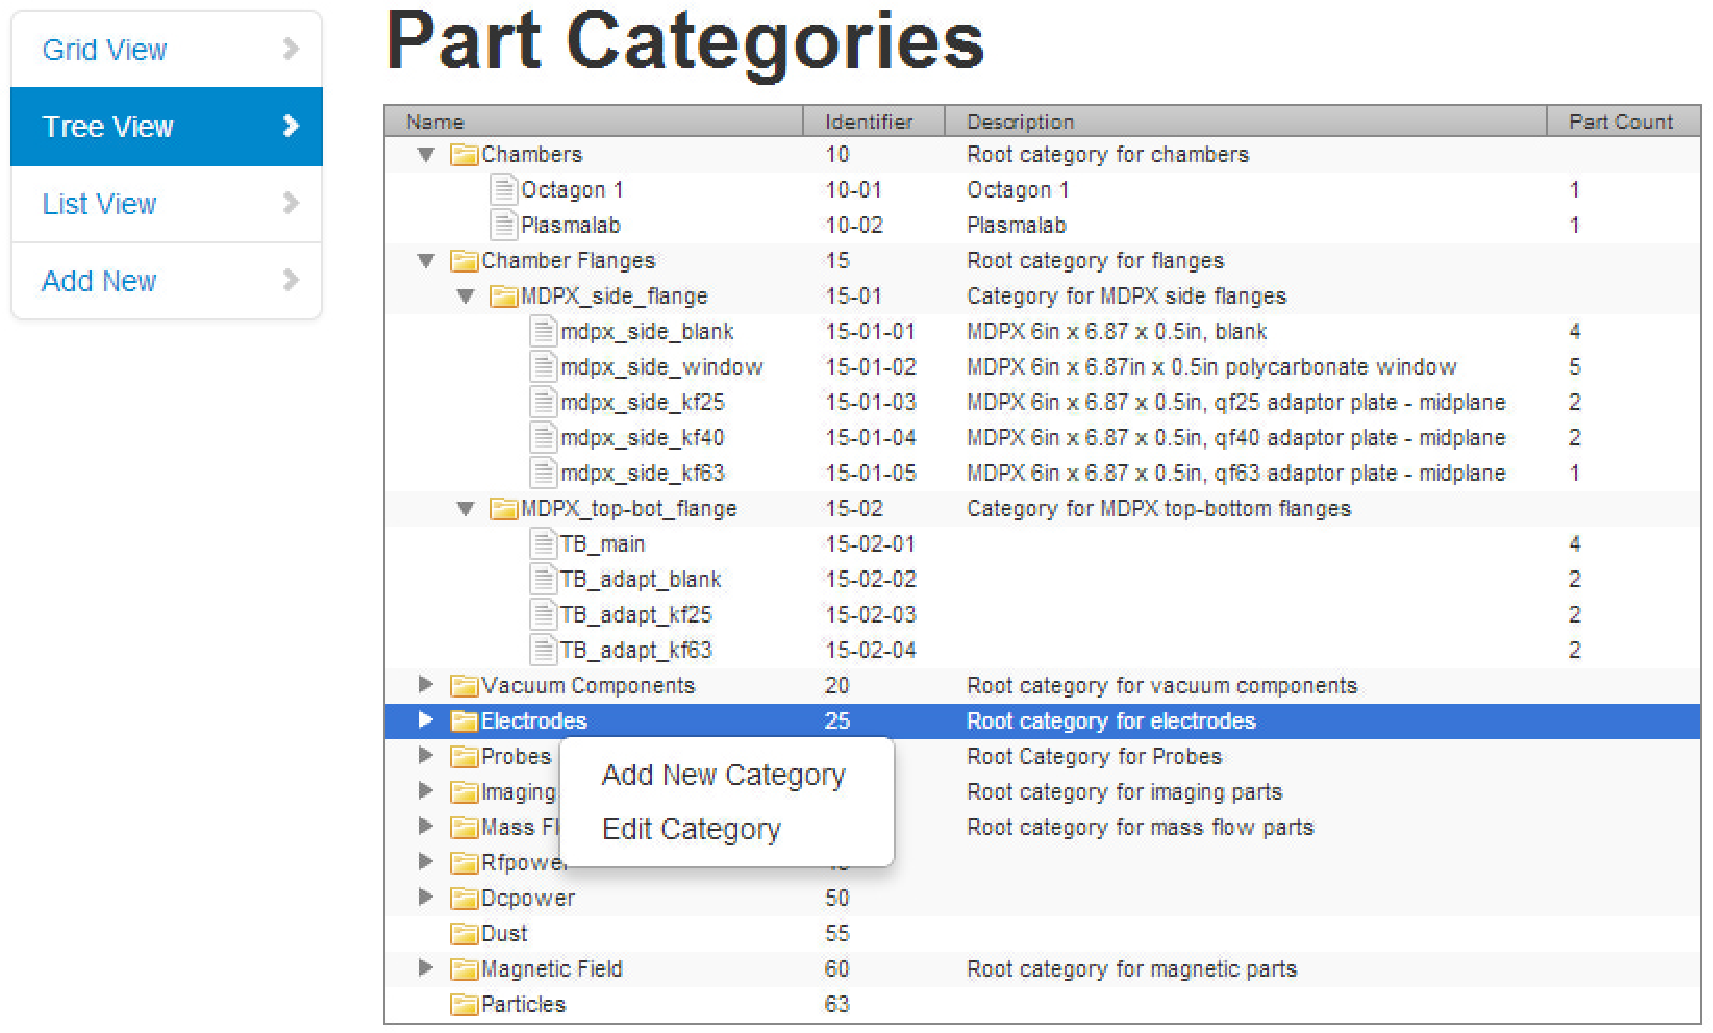
\includegraphics[width=6in]{partcat.pdf}
\caption{Tree view of the part categories.\label{fig:partcat}}
\end{figure}

The web interface is implemented via PHP 5.3 with Yii Framework 1.1. The framework provides agnostic database access; therefore, RDBMS from different vendors can be used as the data store. The RDBMS that are supported include MySQL(what we use), PostgreSQL, SQLite, Microsoft SQLServer.

\subsection{Inserting and Modifying Data}

The interface facilitates entering new data into the database as shown in the Figure~\ref{fig:create_exp_setup}.

\begin{figure}[h]
\centering
\includegraphics[width=6in]{create_experiment_setup.pdf}
\caption{Data entry form and data validation.\label{fig:create_exp_setup}}
\end{figure}

Two ways that the interface make entering and modifying data easier and less error-prone.

The first is that data input form provides selection drop-down menu for data item when possible. The content of these selection menus are usually populated from tables in the database. For example, to insert a new entry into the Experiments table (a experiment group), a researcher and operator user ID is needed. The data entry interface provides a selection menu for these fields so that the user does not have to perform additional step of looking up user IDs. When the data is submitted, the interface inserts the correct user IDs.

The second is that, the interface provides data validation. If a data item does not match a format or validation rule, the data is rejected and will not be saved to the database. The database also enforces data integrity rules. The interface adds a second layer of data integrity and constraint checks.

\subsection{Data Filtering and Searching}

Data filtering is supported in grid views. Figure~\ref{fig:grid_filter} shows the grid view of parts in the system. Users can specify filtering criteria on the columns at the top of the grid view. For string columns, the user can enter the complete or partial search string. For example, to search and researcher with the last name of ``Thomas", the user can enter either ``Thomas" or just ``Thom" as filtering string. For numerical columns, comparison operators ($<$, $>$) can be used in filtering criteria.

\begin{figure}[h]
\centering
\includegraphics[width=6in]{grid_filter.pdf}
\caption{Data Filtering.\label{fig:grid_filter}}
\end{figure}


%\onecolumn
\section{Appendix}
\subsection{Database Tables}\label{app_db_schema}

\begin{figure*}[h]
\centering
\includegraphics[width=6in]{schema.pdf}
\caption{Database schema.\label{fig:schema}}
\end{figure*}

%\begin{figure}[h!]
%\begin{center}
%\includegraphics[width=6in]{schema.pdf}
%\caption{Database schema.\label{fig:schema}}
%\end{center}
%\end{figure}

%\twocolumn

\subsection{Database Column Description}

\begin{table}[h!]
\centering
%\caption{PartCategories Table}\label{tb_tables_in_access}
\begin{tabular}{l p{12cm}}
\multicolumn{2}{c}{\bf PartCategories Table} \\ \hline
{\bf Column} & {\bf Description}\\ \hline
partCatId & Identifier of part category.\\ \hline
name & Display name of part category.\\ \hline
description & A textual description of this part category. \\ \hline
parent & Contains Part Category ID of the parent part category node.\\ \hline
isGroup & Denotes if a Part Category is an intermediate node or a leaf node. \\ \hline
\end{tabular}
\end{table}

\begin{table}[h!]
\centering
%\caption{PartCategories Table}\label{tb_tables_in_access}
\begin{tabular}{l p{12cm}}
\multicolumn{2}{c}{\bf Parts Table} \\ \hline
{\bf Column} & {\bf Description}\\ \hline
serialNum & Unique identifier of each part. TWo physical parts of the same type in the catalog will have the same category ID, but different serial number.\\ \hline
type & Part Category ID.\\ \hline
addedOn & The date and time when the part is added to the catalog. \\ \hline
addedBy & The ID of the user who added the part to the catalog.\\ \hline
\end{tabular}
\end{table}

\begin{table}[h!]
\centering
%\caption{PartCategories Table}\label{tb_tables_in_access}
\begin{tabular}{l p{12cm}}
\multicolumn{2}{c}{\bf GasTypes Table} \\ \hline
{\bf Column} & {\bf Description}\\ \hline
gasTypeId & Unique integer identifier.\\ \hline
name & Name of the gas, e.g. Argon.\\ \hline
\end{tabular}
\end{table}

\begin{table}[h!]
\centering
%\caption{PartCategories Table}\label{tb_tables_in_access}
\begin{tabular}{l p{12cm}}
\multicolumn{2}{c}{\bf DustTypes Table} \\ \hline
{\bf Column} & {\bf Description}\\ \hline
gasTypeId & Unique integer identifier.\\ \hline
name & Name of the particle, e.g. Silica 0.5.\\ \hline
\end{tabular}
\end{table}

\begin{table}[h!]
\centering
%\caption{PartCategories Table}\label{tb_tables_in_access}
\begin{tabular}{l p{12cm}}
\multicolumn{2}{c}{\bf VesselSetups Table} \\ \hline
{\bf Column} & {\bf Description}\\ \hline
vesselSetupId & Unique integer database record identifier.\\ \hline
dateTime & Date and time when this setup was created.\\ \hline
name & A descriptive name of this setup.\\ \hline
\end{tabular}
\end{table}

\begin{table}[h!]
\centering
%\caption{PartCategories Table}\label{tb_tables_in_access}
\begin{tabular}{l p{12cm}}
\multicolumn{2}{c}{\bf SetupParts Table} \\ \hline
{\bf Column} & {\bf Description}\\ \hline
setupPartId & Unique integer database record identifier.\\ \hline
vesselSetupId & The ID of the vessel setup to which this part is attached.\\ \hline
part & Serial number of this part.\\ \hline
parent & The ID of the setup part to which this part is attached.\\ \hline
port & The location on the parent part on which this part is attached.\\ \hline
\end{tabular}
\end{table}

\begin{table}[h!]
\centering
%\caption{PartCategories Table}\label{tb_tables_in_access}
\begin{tabular}{l l p{10.3cm}}
\multicolumn{3}{c}{\bf SetupCameras Table} \\ \hline
{\bf Column} & {\bf Unit} & {\bf Description}\\ \hline
setupPartId & & The ID of the setup part of which this record is describing.\\ \hline
description & & Description of the camera.\\ \hline
positionR & Degree & The R position of the camera.\\ \hline
positionZ & Centimeter & The Z position of the camera.\\ \hline
\end{tabular}
\end{table}

\begin{table}[h!]
\centering
%\caption{PartCategories Table}\label{tb_tables_in_access}
\begin{tabular}{l l p{10.3cm}}
\multicolumn{3}{c}{\bf SetupProbes Table} \\ \hline
{\bf Column} & {\bf Unit} & {\bf Description}\\ \hline
setupPartId & & The ID of the setup part of which this record is describing.\\ \hline
length & Centimeter & The length of the probe.\\ \hline
width & Centimeter & The width of the probe.\\ \hline
\end{tabular}
\end{table}

\begin{table}[h!]
\centering
%\caption{ExperimentSetups Table}\label{tb_tables_in_access}
\begin{tabular}{l l p{7cm}}
\multicolumn{3}{c}{\bf ExperimentSetups Table} \\ \hline
{\bf Column} & {\bf Unit} & {\bf Description}\\ \hline
experimentSetupId & & Unique integer database record identifier.\\ \hline
experimentId & & ID of an record in Experiments table.\\ \hline
dateTime & & Date and time on which this setup was created.\\ \hline
name & & Descriptive name.\\ \hline
description & & Description.\\ \hline
vesselSetupId & & Database ID of the vessel setup of this experiment.\\ \hline
dcVoltageSetpoint & Volt & \\ \hline
dcCurrentSetpoint & Milliamp & \\ \hline
rfPowerSetpoint & Watt & \\ \hline
pressureSetpoint & Volt & \\ \hline
magnet1Setpoint & Amp & \\ \hline
magnet2Setpoint & Amp & \\ \hline
magnet3Setpoint & Amp & \\ \hline
magnet4Setpoint & Amp & \\ \hline
magneticFieldSetpoint & Tesla & \\ \hline
magneticFieldGradientSetpoint & Tesla/Meter & \\ \hline
gasType1 && \\ \hline
gasType2 && \\ \hline
dustType1 && \\ \hline
dustType2 && \\ \hline
\end{tabular}
\end{table}

\begin{table}[h!]
\centering
%\caption{Experiments Table}\label{tb_tables_in_access}
\begin{tabular}{l p{12cm}}
\multicolumn{2}{c}{\bf Experiments Table} \\ \hline
{\bf Column} & {\bf Description}\\ \hline
experimentId & Unique integer database record identifier.\\ \hline
name & Descriptive name of the experiment group.\\ \hline
description & Description of the experiment group.\\ \hline
dateTime & The date and time on which this group was created.\\ \hline
isProgrammed & A boolean flag that signifies if this group of experiment is conducted by a program that iterates through a range of values for a set of paramenters.\\ \hline
description & Description of the experiment group.\\ \hline
researcherId & Foreign key to Users.userId. This means each record in this table has a researcher.\\ \hline
operatorId & Foreign key to Users.userId. This means each record in this table has an operator.\\ \hline
\end{tabular}
\end{table}

\begin{table}[h!]
\centering
%\caption{Measurements Table}\label{tb_tables_in_access}
\begin{tabular}{l l p{8cm}}
\multicolumn{3}{c}{\bf Measurements Table} \\ \hline
{\bf Column} & {\bf Unit} & {\bf Description}\\ \hline
measurementId & & Primary key of this table.\\ \hline
experimentSetupId & & Foreign key to ExperimentSetups.experimentSetupId. This relationship means every measurement is linked with one experiment setup, and every experiment setup has multiple measurements.\\ \hline
dateTime & & Date and time when a record was recorded.\\ \hline
dcVoltage & Volt & Monitored average DC voltage of ...?\\ \hline
dcCurrent & Milliamp & Monitored average DC current of ...?\\ \hline
rfPower & Watt & \\ \hline
massFlow & Volt & \\ \hline
pressure & ? & \\ \hline
magnet1 & Ampere & \\ \hline
magnet2 & Ampere & \\ \hline
magnet3 & Ampere & \\ \hline
magnet4 & Ampere & \\ \hline
magneticField & Tesla & \\ \hline
magneticFieldGradient & Tesla/Meter & \\ \hline
dataPath & & Where the corresponding data is stored.\\ \hline
\end{tabular}
\end{table}

\begin{table}[h!]
\centering
%\caption{PartCategories Table}\label{tb_tables_in_access}
\begin{tabular}{l p{12cm}}
\multicolumn{2}{c}{\bf Users Table} \\ \hline
{\bf Column} & {\bf Description}\\ \hline
userId & Primary key for this table.\\ \hline
email & Email address of this user.\\ \hline
password & Password of the user hashed using md5 without salt.\\ \hline
firstName & First name of the user.\\ \hline
lastName & Last name of the user.\\ \hline
phone & Contact telephone number of the user.\\ \hline
affiliation & Associated organization of the user.\\ \hline
\end{tabular}
\end{table}

\begin{table}[h!]
\centering
%\caption{PartCategories Table}\label{tb_tables_in_access}
\begin{tabular}{l p{12cm}}
\multicolumn{2}{c}{\bf Roles Table} \\ \hline
{\bf Column} & {\bf Description}\\ \hline
roleId & Primary key for this table.\\ \hline
roleName & Name of this role, e.g. Admin.\\ \hline
\end{tabular}
\end{table}

\begin{table}[h!]
\centering
%\caption{PartCategories Table}\label{tb_tables_in_access}
\begin{tabular}{l p{12cm}}
\multicolumn{2}{c}{\bf RolePermissions Table} \\ \hline
{\bf Column} & {\bf Description}\\ \hline
roleId & Foreign key to Roles.roleId. This means for reach \\ \hline
controllerId & Controller identifier of the web interface.\\ \hline
actionId & Action identifier of the web interface.\\ \hline
access & Have value of either ALLOW or DENY. This column specifies whether an operation identified by pair {controllerId, actionId} can be performed by a role.\\ \hline
\end{tabular}
\end{table}
